% Chapter 5
\chapter{Making your own panels}

\section{How you can do that}

\subsection{Required stuffs}

You'll first have to read the NanoXML documentation if you need to use XML in
your panel. Secondly, it is necessary that you use the Javadoc-generated class
references. We will just explain here briefly how to start making your panels.\\

A good thing to do is to read the source code of some IzPack panels. They are
usually \textsl{very} small, so you'll understand easily how to do your owns.\\

\subsection{What you'll have to do}

Extending \IzPack with a panel is something really easy. Actually a panel is a
subclass of \texttt{IzPanel}. So all you have to do is make a subclass too. The
\texttt{IzPanel} class is located in the \texttt{com.izforge.izpack.installer}
package but your panels will have to belong to
\texttt{com.izforge.izpack.panels}.\\

A good thing to make the things easier for you is to work with the IzPack
building Jakarta Ant building process. Just add your class in the source tree
and add the And directives to build your own panels. This way you'll be able to
concentrate on code and nothing else :-)\\

\section{The \texttt{IzPanel} class}

\subsection{UML diagram}

\begin{center}
\fbox{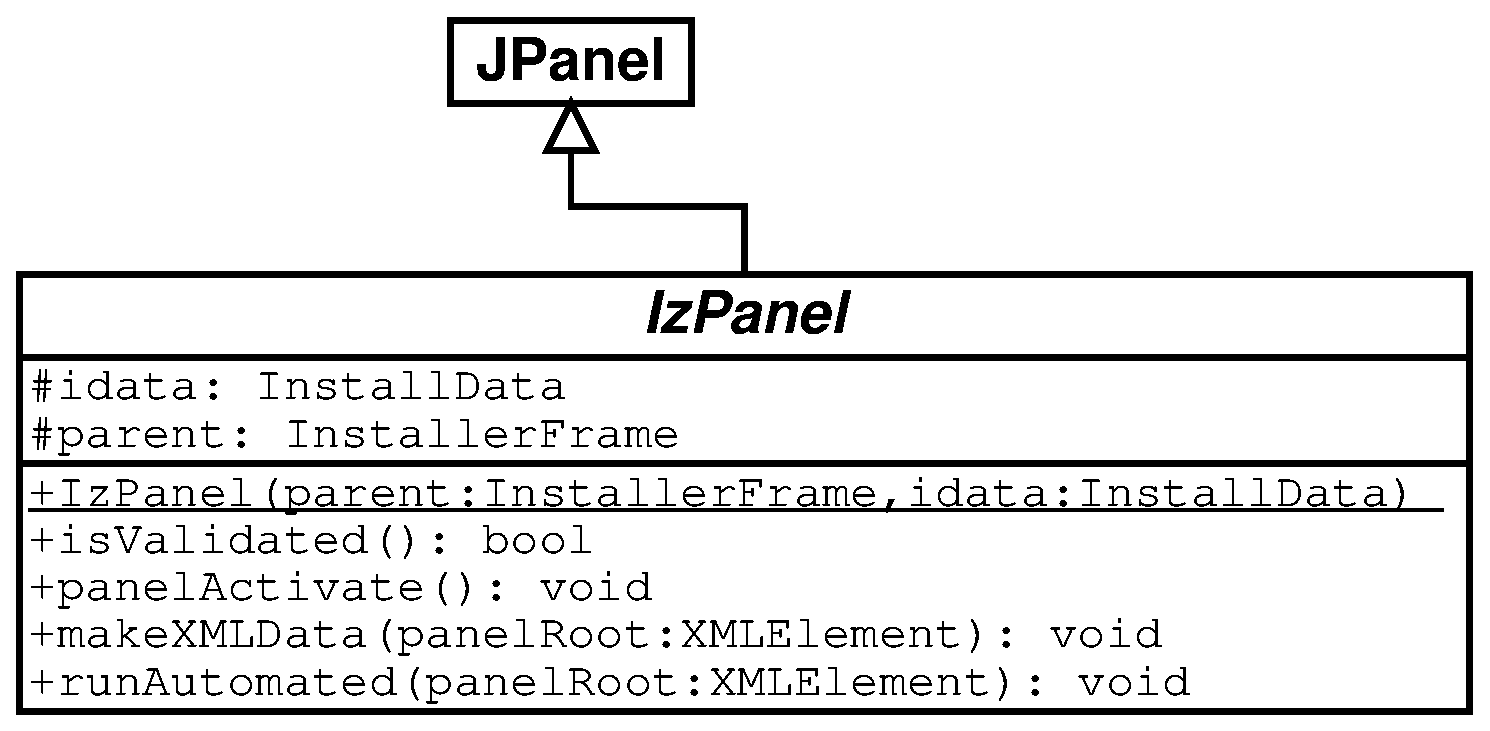
\includegraphics[scale=0.5]{img/ch5-izpanel.eps}}
\end{center}\

\subsection{Description}

The 2 members are : the installer data (refer to the \texttt{InstallData}
Javadoc reference) and the parent installer frame.\\

The methods have the following functions :\\
\begin{itemize}

  \item \textit{(constructor)} : called just after the language selection
  dialog. All the panels are built there and then the installer is shown. So
  take care of the fact that the installer window is \textbf{not} yet visible
  when the panel is created. If you need to do some work when the window exists,
  do it in \texttt{panelActivate}.\\

  \item \texttt{isValidated} returns \texttt{true} if the user is allowed to
  go a step further in the installation process. Returning \texttt{false} will
  lock it. For instance the LicencePanel returns \texttt{true} only if the user
  has agreed with the license agreement. Default is to return \texttt{true}.\\
  
  \item \texttt{panelActivate} is called when the panel becomes active. So
  implement here anything that suits here. Default is to do nothing.\\
  
  \item \texttt{makeXMLData} is called to build the automated installer data.
  Default is to do nothing. \texttt{panelRoot} refers to the node in the XML
  tree where you can save your data. Each panel is given a node. You can
  organize it as you want with the markups you want starting from
  \texttt{panelRoot}. It's that simple.\\
  
  \item \texttt{runAutomated} is called by an automated-mode installation. Each
  panel is called and can do its job by picking the data of the previous
  installation as saved in \texttt{panelRoot} by \texttt{makeXMLData}.\\

\end{itemize}\
